\section{Magdalena Bernat}
\label{sec:magdabernat}
\noindent Co będzie zawierał ten rozdział?

\begin{enumerate}
  \item listę numerowaną
  \item listę nienumerowaną
\end{enumerate}

\noindent ...a także

\begin{itemize}
  \item wyrażenie matematyczne
  \item zdjęcie
  \item tabelę
\end{itemize}


\begin{figure}[htbp]
    \centering
    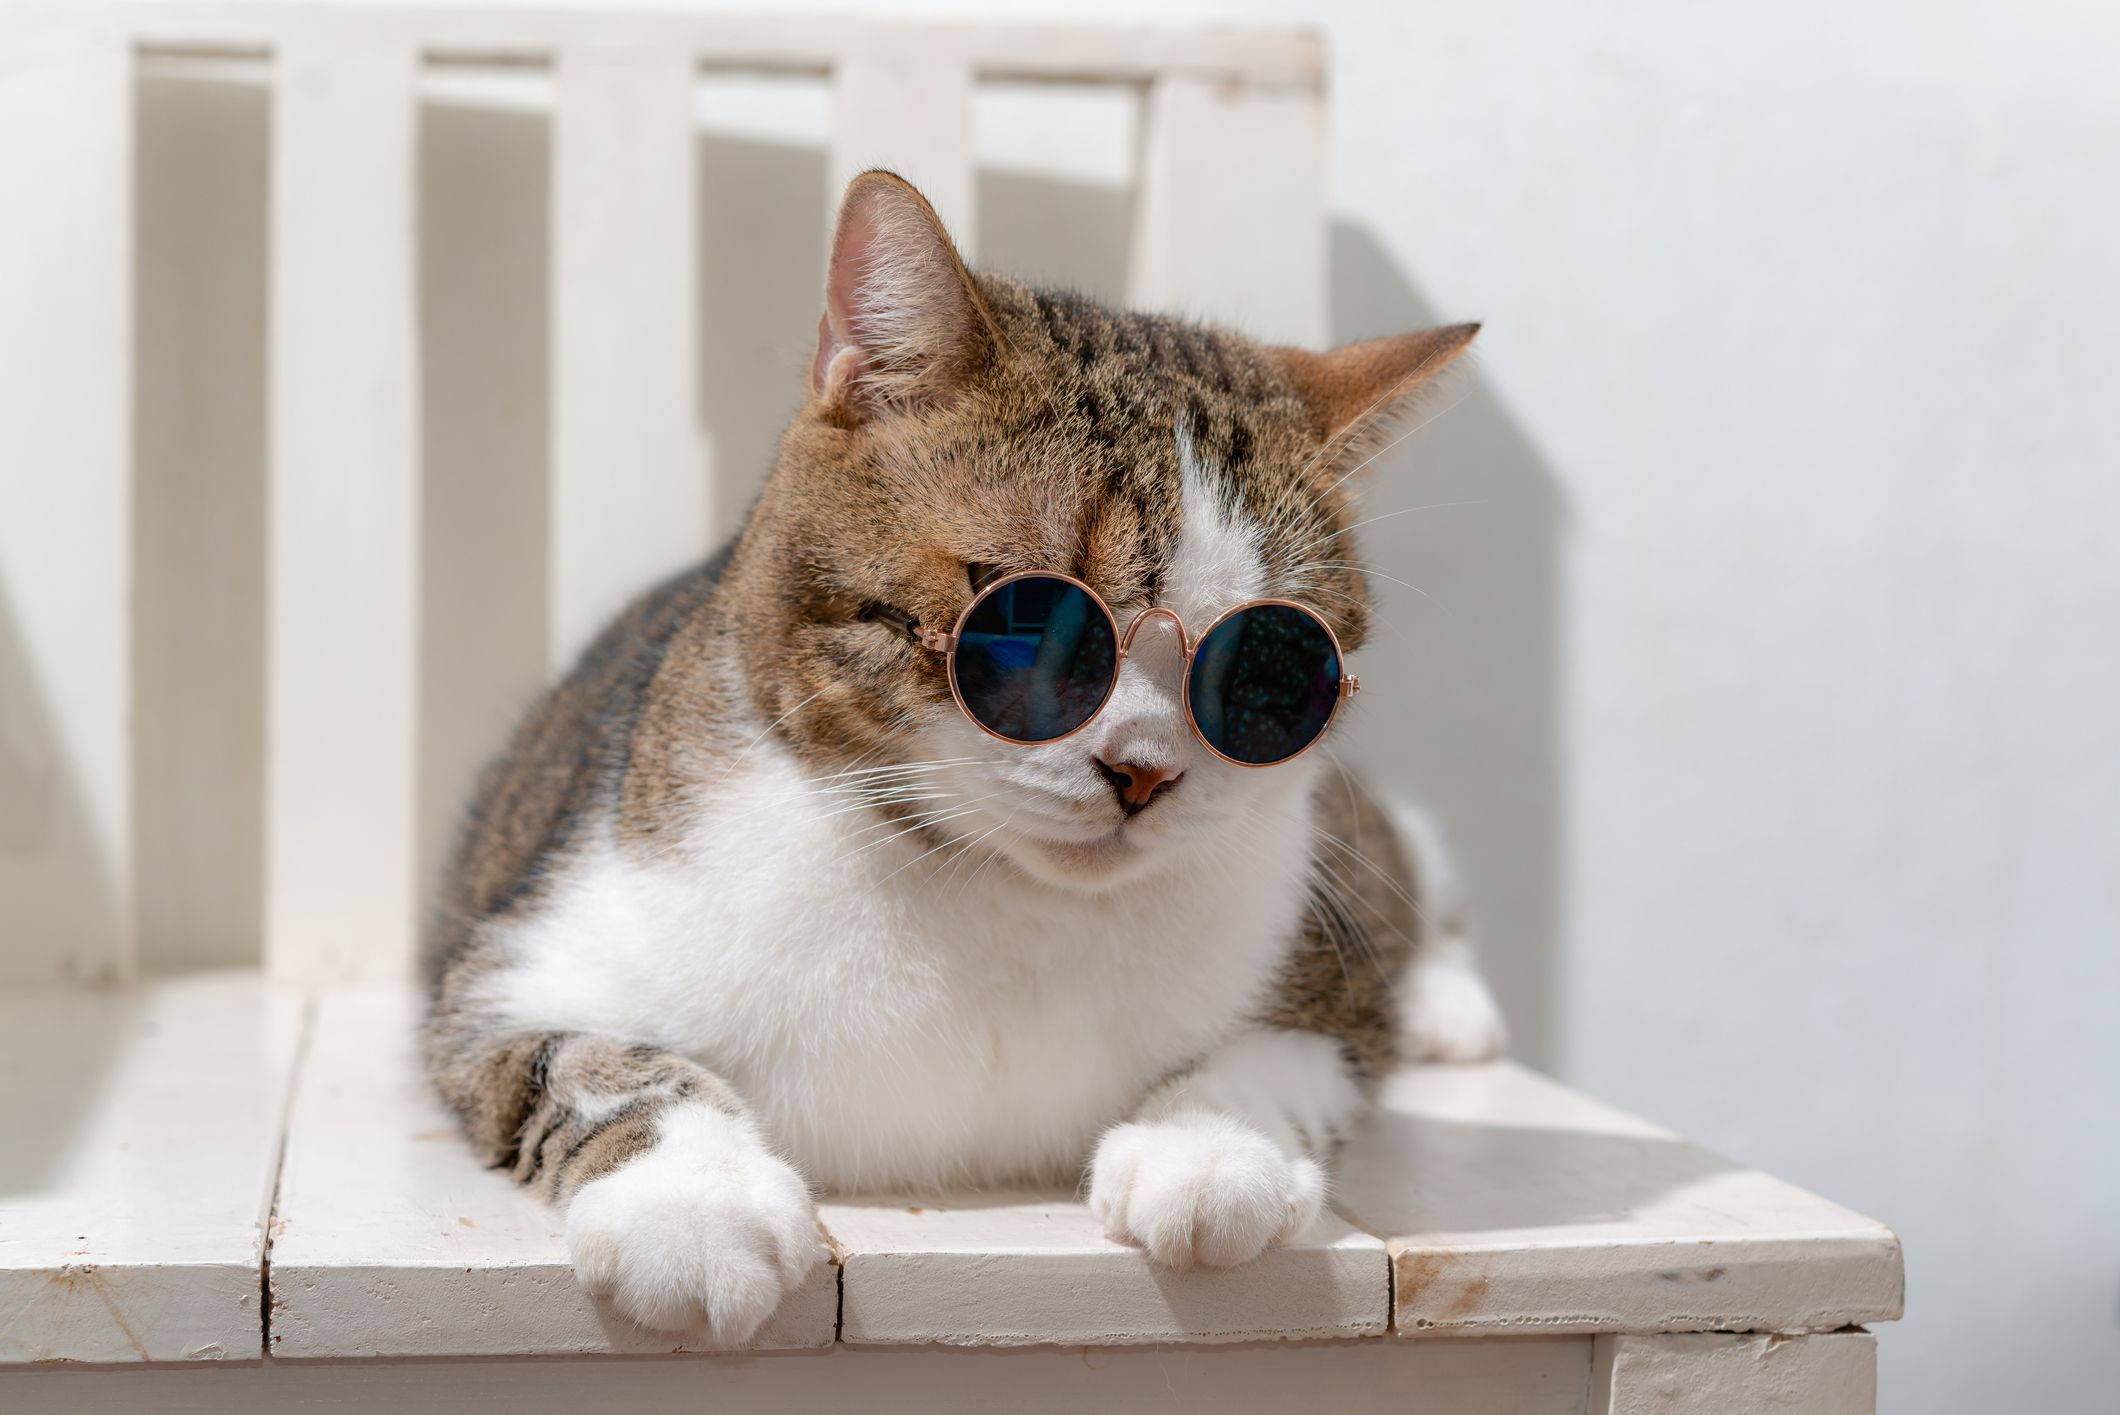
\includegraphics[width=0.6\textwidth]{pictures/cat.jpg}
    \caption{kiciuś}
    \label{fig:kiciuś}
\end{figure}

\noindent Zacznę może od dodania zdjęcia \textbf{kotka}, które można także znaleźć w moim zadaniu na GitHubie :)\\
\noindent Prawdopodobieństwo pojawienia się tego obrazka w obu tych ćwiczeniach można łatwo policzyć ze wzoru:

$$\frac{n!}{k!(n-k)!} = {n}{k}$$

\centering
\noindent\begin{tabular}
{ |p{2cm}|p{2cm}|p{2cm}|p{2cm}|  }
 \hline
 \multicolumn{4}{|c|}{a tutaj jeszcze tabelka} \\
 \hline
 z takimi & zwykłymi & czterema & kolumnami \\
 \hline
 a & d & g & j\\
 b & e & h & k\\
 c & f & i & l\\
 \hline
\end{tabular}


